\chapter{نتایج عملی} \label{chap:experiments}
در این فصل، روش پیشنهادی را روی چند مجموعه دادگان آزمایش کرده و نتایج آن را با سایر روش‌های ارائه شده برای یادگیری بدون برد مقایسه می‌کنیم. ساختار این فصل به این صورت است:
 در بخش \ref{exp:datasets} به معرفی مجموعه دادگان مورد استفاده در آزمایش‌ها می‌پردازیم.
بخش \ref{exp:validation} به شرح الگوریتم اعتبارسنجی برای تنظیم پارامترها می‌پردازد.
 در بخش \ref{exp:cluster} روش خوشه‌بندی نیمه نظارتی از بخش \ref{clustering_method} مورد آزمایش قرار می‌گیرد،
  در بخش \ref{exp:comp} به بررسی تابع مطابقت ارائه شده  در بخش \ref{compatibility_funcion} پرداخته می‌شود
   و در بخش \ref{exp:jeac} روش خوشه‌بندی و نگاشت توام از بخش \ref{jeac} مورد بررسی قرار می‌گیرد.
    در بخش \ref{exp:discussion} نتایج ارائه شده در بخش‌های پیشین مورد تحلیل قرار می‌گیردند و سعی می‌شود دلایل عمل‌کرد بهتر روش پیشنهادی شرح داده شود.
    % در نهایت در بخش \ref{exp:conclusion} جمع‌بندی این فصل صورت می‌گیرد.


\section{مجموعه دادگان مورد استفاده}\label{exp:datasets}
برای آزمایشات عملی ما از چهار مجموعه داده‌ی مرسوم برای سنجش عمل‌کرد روش‌های یادگیری بدون برد استفاده می‌کنیم.

\textbf{\lr{Animal with Attributes (AwA)}} \cite{lampert09}:
این مجموعه داده شامل تصاویر از ۵۰ گونه از پستانداران است. هر دسته توسط یک بردار ویژگی $-85$بعدی توصیف می‌شود. در این مجموعه داده توصیف‌های دسته‌ها هم به صورت مقادیر دودویی به معنای وجود یا عدم وجود آن ویژگی وجود دارند و هم توسط اعداد حقیقی با توجه به میزان وجود آن ویژگی در هر دسته در دسترس هستند. ما از مقادیر پیوسته برای توصیف دسته‌ها استفاده می‌کنیم، چرا که در روش‌های پیشین نشان داده شده که این مقادیر توانای ایجاد تمایز بیشتری دارند \cite{Akata2015}. ما از تقسیم‌بندی آموزش و آزمون انجام شده در خود مجموعه داده استفاده می‌کنیم که در آن ۴۰ دسته به عنوان دسته‌های دیده شده و ۱۰ دسته به عنوان
دسته‌های دیده نشده در نظر گرفته شده‌اند.

\textbf{\lr{aPascal/aYahoo (aPY)}}\cite{farhadi09}:
مجموعه تصاویر
 \lr{VOC 2008} \cite{pascal}
 که شامل ۲۰ دسته است بعنوان دسته‌های دیده شده در نظر گرفته شده است و تصاویر \lr{aYahoo} که شامل ۱۲ دسته هستند به عنوان دسته‌های دیده نشده. برای این دو مجموعه داده، بردار ویژگی‌های $-64$بعدی دودویی برای هر تصویر موجود است. برای بدست آوردن توصیف هر دسته که در مسئله یادگیری بدون برد مورد نیاز است، همانند روش‌های پیشین، روی بردار ویژگی‌های تصاویر هر دسته میان گرفته
 شده است  \cite{lampert09}.


\textbf{\lr{SUN Attribute}} \cite{sun}:
مجموعه تصاویر SUN شامل ۷۱۷ دسته می‌باشد و در این مجموعه برای هر یک از تصاویر یک بردار ویژگی $-102$بعدی موجود است که برای تبدیل آن به توصیف‌های در سطح دسته‌ها، روی بردار ویژگی‌های تصاویر هر دسته میانگین گرفته شده است. ما تقسیم‌بندی آموزش/آزمون انجام گرفته در \cite{jayaraman14} استفاده می‌کنیم که در آن ۱۰ دسته به عنوان دسته‌های دیده نشده در نظر گرفته شده‌اند.

\lr{Caltech UCSD Birds-2011 (CUB)} \cite{cub}:
این مجموعه داده شامل تصاویری از ۲۰۰ گونه از پرندگان است. هر تصویر با ۳۱۲ ویژگی دودویی توصیف می‌شود و توصیف در نظر گرفته شده برای هر دسته میانگین توصیف نمونه‌های آن دسته است. تقسیم‌بندی مورد استفاده برای دسته‌های آموزش و آزمون، دسته‌بندی مورد استفاده در \cite{akata13} است که توسط کارهای بعدی نیز مورد استفاده قرار گرفته است
\cite{sse, Akata2015, Reed2016}.


در تمام مجموعه داده‌ها، برای تصاویر از ویژگی‌های بدست آمده با شبکه‌های عمیق استفاده می‌کنیم چرا که توانایی ایجاد تمایز این ویژگی‌ها نسبت به ویژگی‌های
\textit{کم‌عمق}
سنتی مانند \lr{SIFT}  و \lr{HOG}  بیشتر است.
ویژگی‌های مورد استفاده از  اولین لایه با اتصالات چگال از شبکه ۱۹ لایه‌ی \lr{VGG} \cite{vgg} بدست آمده است. این ویژگی‌ها به صورت عمومی توسط نویسندگان
\cite{sse}
در اختیار قرار گرفته است.
مشخصات مجموعه دادگان مورد استفاده به صورت خلاصه در جدول \ref{tab:datasets} آمده است.
\begin{center}

\begin{table}[ht]
\centering
\caption{مشخصات مجموعه دادگان مورد استفاده در آزمایشات عملی}
\vspace{2mm}
\label{tab:datasets}
\begin{tabular}{|r|c|c|c|c|c|c|}
\hline
 مجموعه داده & ابعاد توصیف‌ & ابعاد تصاویر &  دسته‌های آموزش & دسته‌های آزمون &  نمونه‌های آموزش &  نمونه‌های آزمون \\
\hline
AwA
& 85 & 4096 & 40 & 10 & 24295 & 6180 \\\hline
 aPY
& 64 & 4096 & 20 & 12 & 12695 & 2644 \\\hline
CUB-2011
& 312 & 4096 & 150 & 50 & 8855 & 2933 \\ \hline
 SUNA
& 102 & 4096 & 707 & 10 & 14140 & 200 \\
\hline
\end{tabular}
\end{table}
\end{center}


\section{نحوه‌ی اعتبارسنجی}\label{exp:validation}
برای تعیین فراپارامترهای مورد استفاده در روش‌های ارائه شده، یعنی  فراپارامتر $\beta$ در رابطه \eqref{eq:nn_loss}،
 $\gamma$ در رابطه \eqref{eq:d_definition} و مقادیر $\lambda$ و $\gamma$ در رابطه \eqref{eq:joint} از یک الگوریتم اعتبار سنجی مرسوم در روش‌های یادگیری بدون برد استفاده می‌شود.
در این حالت تعدادی از دسته‌های آموزش به عنوان دسته‌های اعتبارسنجی در نظر گرفته شده و اعتبار سنجی به این صورت در انجام می‌شود که آموزش روی سایر دسته‌ها صورت گرفته و روی دسته‌های اعتبارسنجی که دیده نشده فرض شده‌اند، سنجیده می‌شود. بدیهی است که مجموعه‌ دسته‌های آزمون اصلی در این روند به هیچ صورتی مورد استفاده قرار نمی‌گیرند. وقتی مقادیر فراپارامترها تعیین شد، روش روی کل دسته‌های دیده‌شده آموزش می‌بیند. ما تعداد دسته‌های اعتبارسنجی را برای هر مجموعه به گونه‌ای انتخاب کردیم که نسبت تعداد دسته‌های اعتبارسنجی به سایر دسته‌های آموزش برابر نسبت تعداد دسته‌های آزمون به کل دسته‌های آموزش باشد. برای اعتبار سنجی الگوریتم به ازای هر مقدار فراپامتر ۱۰ بار با انتخاب تصادفی دسته‌های اعتبارسنجی از دسته‌های آزمون اجرا شده و عمل‌کرد روی این ۱۰ حالت میانگین گرفته شده است.
%
\section{پیش‌بینی ویژگی با شبکه عصبی چند وظیفه‌ای}
\begin{table}[ht]
\caption [دقت دسته‌بندی با شبکه عصبی چندوظیفه‌ای]{
مقایسه دقت دسته‌بندی چنددسته‌ای روش پیشنهادی با سایر روش‌ها. نتایج بر اساس نوع ویژگی مورد استفاده برای تصاویر دسته‌بندی شده‌اند. جدول شامل دقت دسته‌بندی چنددسته‌ای به صورت 
(میانگین $\pm$ انحراف معیار) است. نتایج سایر روش‌ها از مقالاتی که روش در آن‌ها ارائه شده نقل شده و آزمایش‌ها توسط ما تکرار نشده است. 
}
\label{tab:nn}
\begin{tabular}{|r|c|c|c|c|}
\hline
روش  & AwA & CUB-2011 & aPY & SUNA \\
\hline
\lr{Jayaraman and Grauman}  \cite{jayaraman14}  & $43.01 \pm 0.07$ &                 & $26.02 \pm 0.05$        & $56.18 \pm 0.27$ \\
\hline
\lr{Lampert et al \cite{lampert09} (DAP)}	&$57.5$ &		& 		& $22.2$ \\
\hline
\lr{Lampert et al \cite{lampert09} (IAP)}	&$44.5$ &		& 		& $18.0$ \\
\hline
پیشنهادی (بخش \ref{nn})
                      & \textbf{${74.52 \pm 1.93}$}  & \textbf{${33.76 \pm 0.21}$} & \textbf{${31.88}$} & \textbf{ ${69.5}$} \\
\hline
\end{tabular}

\end{table}
در این بخش، شبکه‌ی عصبی معرفی شده در بخش \ref{nn} با سایر روش‌های پیش‌بینی ویژگی مقایسه می‌کنیم.
 اندازه دسته‌ها\LTRfootnote{batch size} در جریان آموزش برابر ۱۲۸ در نظر گرفته شده است. 
پیش از آموزش شبکه به صورت کامل، از یک روند پیش‌آموزش استفاده کرده‌ایم که در آن تنها نمونه‌های آموزش به شبکه وارد شده و خروجی با توصیف صحیح آن‌ها مقایسه می‌شود (نیمه‌ی چپ تصویر
\ref{fig:nn2}).
تعداد تکرارها در جریان پیش آموزش ۱۵ و در آموزش کلی شبکه ۳۰ در نظر گرفته شده است چرا که روند همگرایی در همین تعداد تکرار اتفاق می‌افتد و افزایش تکرارها تاثیری در بهبود نتایج ندارد. 
آموزش شبکه برای مجموعه دادگان \lr{AwA} و \lr{CUB-2011} از الگوریتم بهینه‌سازی \lr{adam} 
\cite{adam}
استفاه شده است. برای مجموعه دادگان \lr{SUN} و \lr{aPY} الگوریتم 
\lr{adadelta} \cite{adadelta}
مورد استفاده قرار گرفته.
 پیاده‌سازی این شبکه با استفاده از ابزارهای متن باز 
\lr{Theano} \cite{theano}
و 
 \lr{Keras} \cite{keras}
صورت گرفته است. 

جدول \ref{tab:nn} دقت دسته‌بندی چند دسته‌ای با استفاده از این روش را به همراه نتایج سایر روش‌های با رویکرد پیش‌بینی ویژگی نشان می‌دهد. همان‌طور که مشاهده می‌شود، استفاده از این شبکه عمل‌کرد بهتری نسبت به سایر روش‌های پیش‌بینی ویژگی داشته است.

\section{بررسی خوشه‌بندی نیمه‌نظارتی}\label{exp:cluster}
\begin{table}[ht]
\centering
\caption[بررسی عمل‌کرد خوشه‌بندی نیمه‌نظارتی پیشنهاتی]{
امتیاز معیار دقت (٪) تخصیص خوشه‌ها که با رای‌گیری روی برچسب‌های صحیح به شماره دسته تبدیل شده است؛ بر روی چهار مجموعه داده مورد استفاده در یادگیری بدون برد. نتایج روش پیشنهادی به صورت 
\textit{ میانگین $\pm$ انحراف معیار }
برای سه اجرا گزارش شده‌است.}
\vspace*{2mm}
  \label{tab:clustering}
\begin{tabular}{|r|c|c|c|c|}
\hline
روش خوشه‌بندی & AwA & CUB-2011 & aPY & SUNA \\
\hline
k-means                             &  ${65.80}$                 & ${35.61}$           & ${65.37 }$               & ${17.49 }$   \\
\hline
پیشنهادی (بخش \ref{clustering_method})
                      & \textbf{${70.74\pm 0.32}$}  & \textbf{${42.63\pm 0.07}$} & \textbf{${69.93\pm 3.4}$} & \textbf{ ${45.50 \pm 1.32}$} \\
\hline
\end{tabular}
\vspace{2mm}
\end{table}

در این بخش به بررسی عمل‌کرد روش خوشه‌بندی نیمه‌نظارتی ارائه شده در بخش \ref{clustering_method} می‌پردازیم. برای این منظور روش ارائه شده را روی هر مجموعه داده اجرا کرده، خوشه‌های مربوط به دسته‌های آزمون را کنار گذاشته  و هر یک از خوشه‌های دیگر را به یک دسته از دسته‌های آزمون نسبت می‌دهیم. برای این کار در هر خوشه بر اساس برچسب صحیح نمونه‌ها رای‌گیری می‌شود و برچسبی که بیشتر اعضای آن خوشه آن را دارا هستند به کل اعضای خوشه نسبت داده می‌شود. نتیجه با برچسب‌های صحیح مقایسه شده و دقت چنددسته‌ای\LTRfootnote{mulit-class ccurary} در جدول \ref{tab:clustering} گزارش شده است.
 برای مقایسه عمل‌کرد، آزمایش مشابهی را با روش \lr{k-means} اجرا می‌کنیم. به این صورت که  الگوریتم \lr{k-means} را با $k=n_s + n_u$ اجرا کرده و با هر خوشه با رای‌گیری برچسب یکی از دسته‌های دیده نشده را نسبت می‌دهیم. نتایج مربوط به این آزمایش نیز در جدول \ref{tab:clustering} گزارش شده است.

\section{بررسی دقت دسته‌بندی بدون برد}\label{exp:comp}
در این بخش عمل‌کرد روش‌های پیشنهادی ارائه شده برای یادگیری بدون برد را با اخیرترین روش‌های دیگر که در فصل \ref{chap:lr} مقایسه می‌کنیم. معیار مورد استفاده برای این مقایسه که پرکاربردترین معیار در این زمینه است، دقت دسته‌بندی چنددسته‌ای است.
\subsection{دسته‌بندی ساده با تابع مطابقت مبتنی بر خوشه‌بندی}
روش نخست پیشنهادی،  در بخش \ref{simple_method}  معرفی شد و مراحل آن در الگوریتم \ref{alg:simple} ذکر شده است. این روش مبتنی بر یک خوشه‌بندی روی داده‌های آزمون بود و با استفاده از یک نگاشت خطی از فضای توصیف دسته‌ها به فضای تصاویر، مرکز هر خوشه را به یک دسته‌هی دیده نشده منتسب می‌کرد. بر اساس تابع مطابقت پیشنهادی (بخش \ref{compatibility_funcion})، تمام اعضای هر خوشه همان برچسبی که مرکزشان دریافت کرده را دریافت می‌کند.

این روش با استفاده از دو نوع خوشه‌بندی آزمایش شده است. یکی خوشه‌بندی نیمه‌نظارتی پیشنهادی که نتایج این حالت با عنوان 
\textit{پیشنهادی (خوشه‌بندی + تابع مطابقت) }
در جدول \ref{tab:results} آمده است.
 برای بررسی تاثیر خوشه‌بندی ارائه شده یک نسخه دیگر از این روش که در آن از خوشه‌بندی \lr{k-means} بجای خوشه‌بندی پیشنهادی استفاده شده است نیز مورد آزمایش قرار گرفته است. نتایج مربوط به این روش با عنوان
\textit{ پیشنهادی (تابع مطابقت + \lr{k-means} ) }
آمده است. نتایج ارائه شده حاصل سه بار اجرا هستند که به صورت
\textit{ میانگین $\pm$ انحراف معیار }
بیان شده‌اند. همان‌گونه که از نتایج مشخص است، استفاده از خوشه‌بندی نیمه‌نظارتی ارائه شده همواره نتایج بهتری نسبت به استفاده از خوشه‌بندی  \lr{k-means} تولید خواهد کرد.
\subsection{ خوشه‌بندی و یادگیری نگاشت توام}\label{exp:jeac}
روش پیشنهادی دوم که در بخش \ref{jeac} ارائه شد به خوشه‌بندی و یادگیری نگاشت توام می‌پرداخت و برچسب نمونه‌های آزمون در آن به طور مستقیم در جریان آموزش بدست می‌آید.
تنظمیات آزمایش برای روش خوشه‌بندی و نگاشت توام مانند حالت قبل سه بار اجرا و گزارش نتایج به صورت \textit{ میانگین $\pm$ انحراف معیار } است. دو نوع  مقدار دهی اولیه انجام شده است. یکی همان‌طور که در بخش \ref{jeac} بیان شد، مقدار دهی $R$ که با استفاده از الگوریتم
\ref{alg:simple}
انجام می‌شود. نتایج مربوط به این حالت در جدول  \ref{tab:results} با عنوان
\textit{ پیشنهادی (توام، مقداردهی $R$)}
آمده‌اند. یک مقدار دهی دیگر شروع بهینه‌سازی تناوبی در الگوریتم
\ref{alg:jeac}
 با مقداردهی $D$ است که توسط رابطه
\eqref{eq:d_answer}
صورت گرفته است. نتایج مربوط به این حالت با عنوان
\textit{پیشنهادی (توام، مقداردهی $D$)}
آمده‌اند. مقایسه نتایج مربوط به این دو نحوه‌ی مقداردهی اولیه نشان می‌دهد که استفاده از روش پیشنهادی الگوریتم \ref{alg:simple}  برای رسیدن به دقت بالا ضروری است.

\subsection{روش‌های مورد مقایسه}\label{exp:other_methods}
سایر روش‌هایی که در جدول  \ref{tab:results} برای مقایسه آورده شده‌اند، روش‌هایی هستند که بالاترین دقت‌های دسته‌بندی را در دسته‌بندی بدون برد با استفاده از توصیف‌های به صورت بردار ویژگی دارا هستند.
روش‌های ارائه شده در 
\cite{li15max, semi15, Kodirov2015}
از این جهت که \textit{نیمه‌نظارتی} هستند، یعنی از  نمونه‌های آزمون نیز در زمان آموزش استفاده می‌کنند، با روش‌های ما بیشترین نزدیکی را دارند. البته در 
\cite{li15max, semi15}
از ویژگی‌های کم‌عمق برای تصاویر استفاده شده است که توانایی جداسازی دسته‌ها در آن بسیار پایین‌تر از ویژگی‌های بدست آمده از شبکه‌های عصبی عمیق است که در روش‌های پیشنهادی ما مورد استفاده قرار گرفته است. روش‌های 
\cite{Akata2015, Xian2016}
با استفاده از توابع هزینه‌ی بیشترین حاشیه سعی در یادگیری نگاشت از هر دو فضای تصاویر و توصیف دسته‌ها به فضای مشترک دارند. این روش‌ها از ویژگی‌های شبکه‌ی عمیق 
\lr{GoogleNet}
 \cite{googlenet}
 برای استخراج ویژگی استفاده می‌کنند. ابعاد ویژگی‌های بدست آمده ۱۰۲۴ است که بعد کمتری نسبت به ویژگی‌های ۴۰۹۶-بعدی استخراج شده از شبکه ۱۹ لایه‌ی vgg دارد و توانایی جداسازی دسته‌ها در آن پایین‌تر است. همان‌طور که مشاهده می‌شود استفاده از این ویژگی‌های با بعد بیشتر عمل‌کرد روش ارائه شده در \cite{Akata2015} را بهبود داده است.
 
 روش‌هایی که بهترین نتایج را در میان روش‌های رقیب کسب کرده‌اند، روش ارائه شده در \cite{sse} و تعمیم آن در \cite{agnostic}  هستند. هرچند این روش‌ها نیمه‌نظارتی نیستند و تنها از نمونه‌های آموزش برای یادگیری نمایش تصاویر و توصیف دسته‌ها در یک فضای مشترک، که فضای هیستوگرام دسته‌های دیده شده است استفاده می‌کنند، نتایج بهتری نسبت به روش‌های نیمه‌نظارتی پیشین در \cite{li15max, semi15, Kodirov2015} کسب کرده‌اند. این مسئله می‌توان نشان‌گر یک مسیر مناسب در ترکیب روش پیشنهادی در این پژوهش با فضای مشترک مورد استفاده در آن روش‌ها برای کارهای آتی باشد.

\begin{table}[ht]
\caption [مقایسه دقت دسته‌بندی]{
مقایسه دقت دسته‌بندی چنددسته‌ای روش پیشنهادی با سایر روش‌ها. نتایج بر اساس نوع ویژگی مورد استفاده برای تصاویر دسته‌بندی شده‌اند. جدول شامل دقت دسته‌بندی چنددسته‌ای به صورت 
(میانگین $\pm$ انحراف معیار) است. نتایج سایر روش‌ها از مقالاتی که روش در آن‌ها ارائه شده نقل شده و آزمایش‌ها توسط ما تکرار نشده است. نتایج روش‌های پیشنهادی حاصل سه اجرا هستند.
}
\vspace{4mm}
 \label{tab:results}
 {\footnotesize
\begin{tabular}{|r|r|c|c|c|c|}
\hline
ویژگی تصاویر & روش  & Animals with Attributes & CUB-2011 & aPascal-aYahoo & SUN \\
\hline
{کم‌عمق}
& \lr{Li and Guo } \cite{li15max}                 &  $38.2 \pm 2.3$   &                 &                         & $18.9 \pm 2.5$ \\
& \lr{Li \textit{et al.}}~\cite{semi15}                    &  $40.05\pm 2.25$ &                 &   $24.71 \pm 3.19$       &     \\
& \lr{Jayaraman and Grauman}  \cite{jayaraman14}  & $43.01 \pm 0.07$ &                 & $26.02 \pm 0.05$        & $56.18 \pm 0.27$ \\
\hline
{GoogleNet}
& \lr{Akata \textit{et al.}}~\cite{Akata2015}              & $66.7$          & $50.1$            &                         & \\
%& \lr{Changpinyo \textit{et al.}}~\cite{Synthesized}       & $72.9$           & $54.5$            &                         & $62.7$ \\
& \lr{Xian \textit{et al.}}~\cite{Xian2016}                & $71.9$            & $45.5$            &                         & \\
\hline
{VGG-19}
&\lr{ Khodirov \textit{et al.}} \cite{Kodirov2015}
                                            & $73.2$            &  $39.5$           & $26.5$                    &  \\
& \lr{Akata \textit{et al.}}~\cite{Akata2015}              & $61.9$            &  $50.1$           &                         & \\
& \lr{Zhang and Saligrama}  \cite{sse}            &  $76.33 \pm 0.53$ & $30.41 \pm 0.20$ &   $46.23 \pm 0.53$      & $82.50 \pm 1.32$    \\
& \lr{Zhang and Saligrama} \cite{agnostic}       &  $80.46 \pm 0.53$ & $42.11 \pm 0.55$ &   \textbf{$50.35 \pm 2.97$}      & $83.83 \pm 0.29$    \\
&  پیشنهادی (ساده + \lr{k-means})
                          & $86.34 \pm 0.13$               & $52.48 \pm 0.60$              & $48.03 \pm 1.56$              & $75.75 \pm 1.06$ \\
& پیشنهادی (ساده)
                        & $86.38 \pm 0.56$              & $ 53.10\pm 0.43 $             & $48.00 \pm 0.69$              &$ 80.66 \pm 0.76$ \\
& پیشنهادی (توام، مقداردهی $D$)
                     & $83.03$                        & $57.55$                       & $42.62$          & $72.50$\\
& پشنهادی (توام، مقداردهی $R$)
                     & \textbf{\em $88.64 \pm 0.04$}  & \textbf{\em $58.80 \pm 0.64$} & $49.77 \pm 2.02$ & \textbf{\em $86.16 \pm 0.57$} \\
\hline
\end{tabular}
}
\end{table}

\section{تحلیل نتایج}\label{exp:discussion}
برای تحلیل کارایی روش قسمت‌های مختلف آن و تاثیر هر یک  روی یک مجموعه داده واقعی در شکل
\ref{fig:discussion}
 نشان داده شده است. نتایج مربوط به اجرای روش روی تمام مجموعه دادگان AwA است، ولی برای این که تغییرات در شکل قابل دنبال کردن باشند تنها چهار دسته در  تصویر نشان داده شده‌اند که دو دسته از آن‌ها دسته‌های دیده شده و دو دسته از دسته‌های دیده نشده هستند. در تصویر
\ref{fig:null}
دسته‌های دیده شده به صورت رنگی و دسته‌های دیده نشده با رنگ سیاه مشخص شده‌اند. در تصویر
\ref{fig:truth}
برچسب‌های صحیح برای دسته‌های دیده نشده نیز با رنگ مشخص شده است. در تصویر
\ref{fig:knn}
توصیف دسته‌ها با استفاده از نگاشت $D$ از رابطه \eqref{eq:d_answer} به فضای تصاویر برده شده (نماد ستاره) و سپس نمونه‌های آزمون با استفاده از دسته‌بند نزدیکترین همسایه دسته‌بندی شده‌اند، نمونه‌هایی که رنگ قرمز دارند به دسته‌ای غیر از چهار دسته‌ی موجود در تصویر دسته‌بندی شده‌اند. تصویر 
\ref{fig:kmeans}
حاصل دسته‌بندی به شیوه‌ی روش ارائه شده در بخش \ref{simple_method} است که در آن از خوشه‌بندی \lr{k-means} و تابع مطابقت پیشنهادی استفاده شده است. تصویر
\ref{fig:clustering}
مشابه حالت قبل است با این تفاوت که در آن از خوشه‌بندی نیمه‌نظارتی پیشنهادی به‌جای \lr{k-means} استفاده شده است. در تصویر
\ref{fig:jeac}
دسته‌بندی و یادگیری نمایش توصیف دسته‌ها در فضای تصاویر (ستاره‌ها) به صورت توام با روش پیشنهادی بخش \ref{jeac} صورت گرفته است.
همان‌طور که در تصاویر
\ref{fig:kmeans} و \ref{fig:clustering}
مشخص است، استفاده از  تابع مطابقت معرفی شده در بخش \ref{compatibility_funcion} برای دسته‌بندی بسیار موفق‌تر از دسته‌بند نزدیک‌ترین همسایه عمل می‌کند و اطلاعات غیر نظارتی موجود در نمونه‌های آزمون دقت  دسته‌بندی را بهبود می‌دهد. هم‌چنین برتری روش خوشه‌بندی پیشنهادی در تصویر \ref{fig:clustering} قابل مشاهده است. در تصاویر \ref{fig:knn} تا \ref{fig:clustering} که از نگاشت  \eqref{eq:d_answer} برای تصویر کردن توصیف‌ها در فضای تصاویر استفاده شده است، مشکل جابجایی دامنه کاملا قابل رویت است، یعنی برای دسته‌های دیده شده توصیف‌ها به صورت مناسبی در مرکز نمونه‌های آن دسته نگاشته شده‌اند حال آن که برای دسته‌های دیده نشده جابجایی وجود دارد و توصیف‌های آن‌ها از نمونه‌هاشان فاصله گرفته‌اند؛ اما در تصویر
\ref{fig:jeac}
که از روش خوشه‌بندی و یادگیری نگاشت توام استفاده شده است این مشکل برطرف شده است و توصیف‌های دسته‌های دیده نشده نیز مانند دسته‌های دیده شده به مرکز نمونه‌های مربوط به خودشان نگاشته شده‌اند.

\begin{figure}[t]
  \centering
  \begin{subfigure}[b]{0.27\linewidth}
    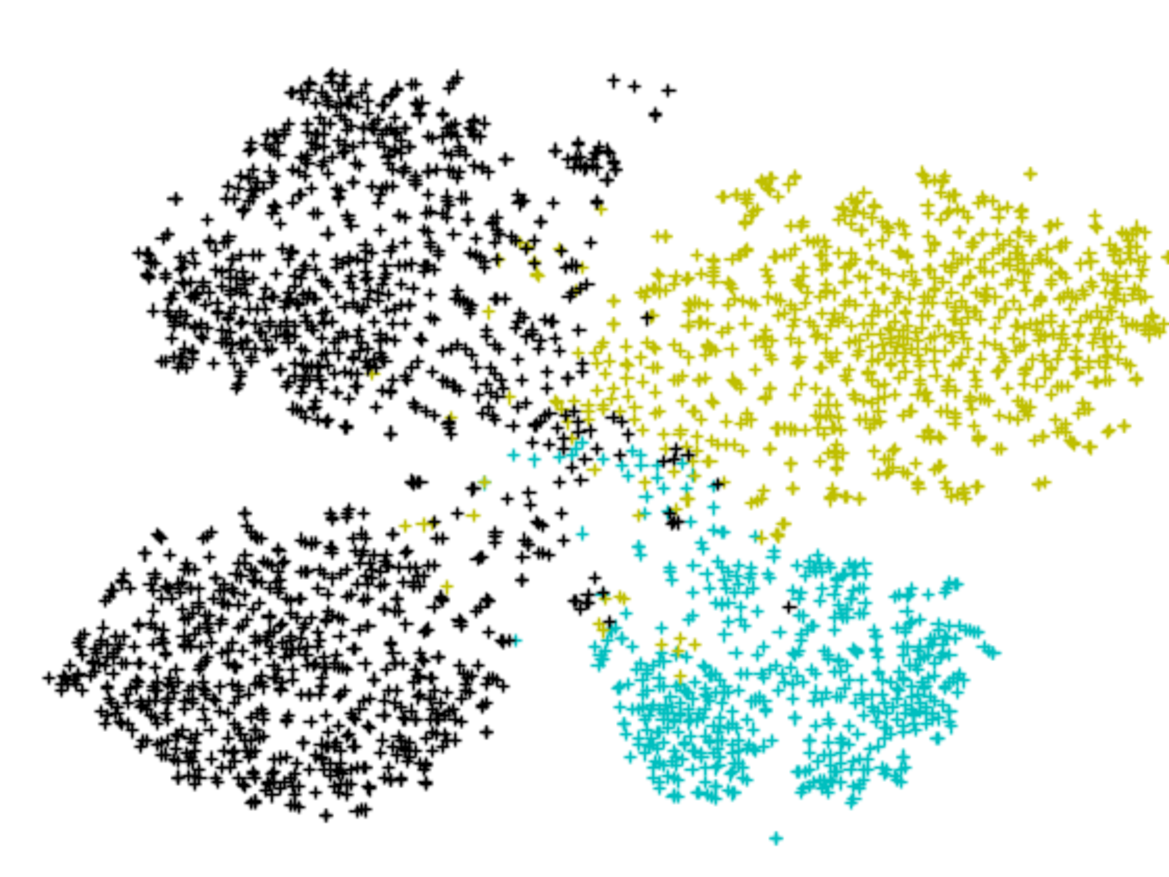
\includegraphics[width=\linewidth]{images/none}
    \caption{}
    \label{fig:null}
  \end{subfigure}
%
  \begin{subfigure}[b]{0.27\linewidth}
    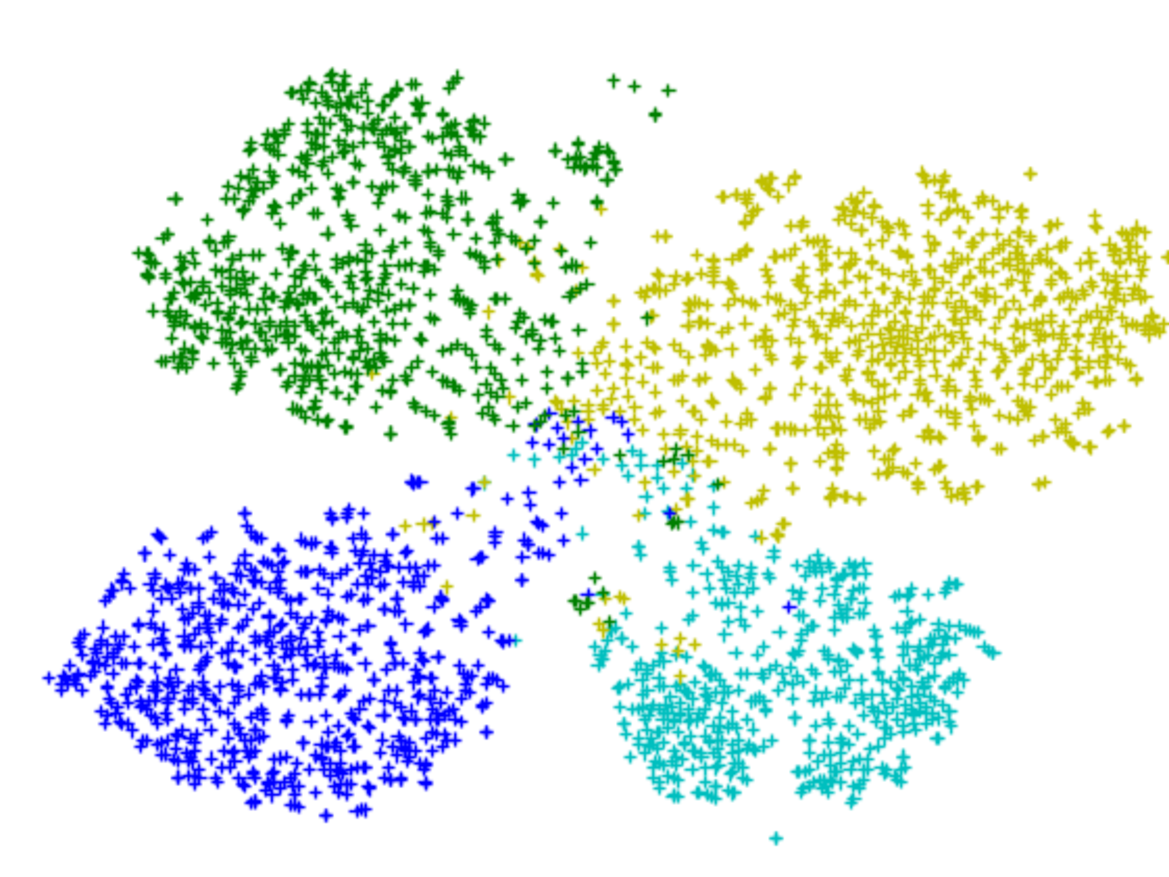
\includegraphics[width=\linewidth]{images/truth}
    \caption{}
% \caption{Points colored according to their ground truth labels}
    \label{fig:truth}
  \end{subfigure}
%
  \begin{subfigure}[b]{0.27\linewidth}
    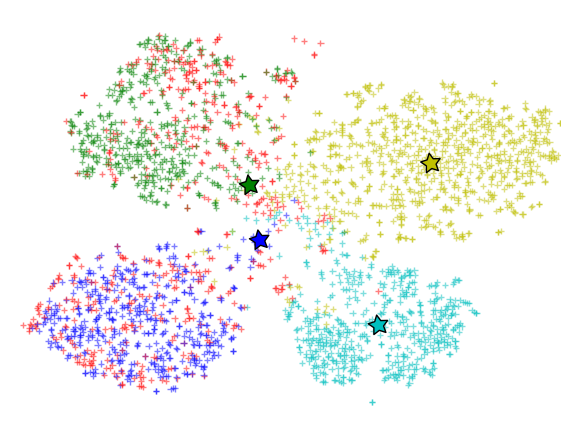
\includegraphics[width=\linewidth]{images/knn}
    % \caption{Signatures mapped to image spacing using Eq. \eqref{eq:dic} and denoted by stars. Then classification done using nearest neighbor}
    \caption{}
\label{fig:knn}
  \end{subfigure}
%
  \begin{subfigure}[b]{0.27\linewidth}
    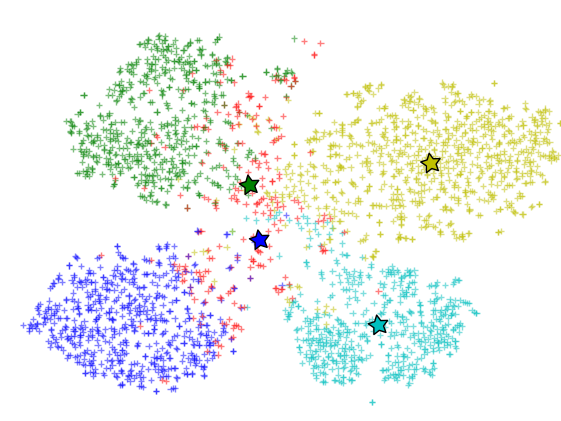
\includegraphics[width=\linewidth]{images/kmeans}
    % \caption{Stars as previous. Classification done by our compatibility function on cluster assignments from k-means}
    \caption{}
\label{fig:kmeans}
  \end{subfigure}
%
  \begin{subfigure}[b]{0.27\linewidth}
    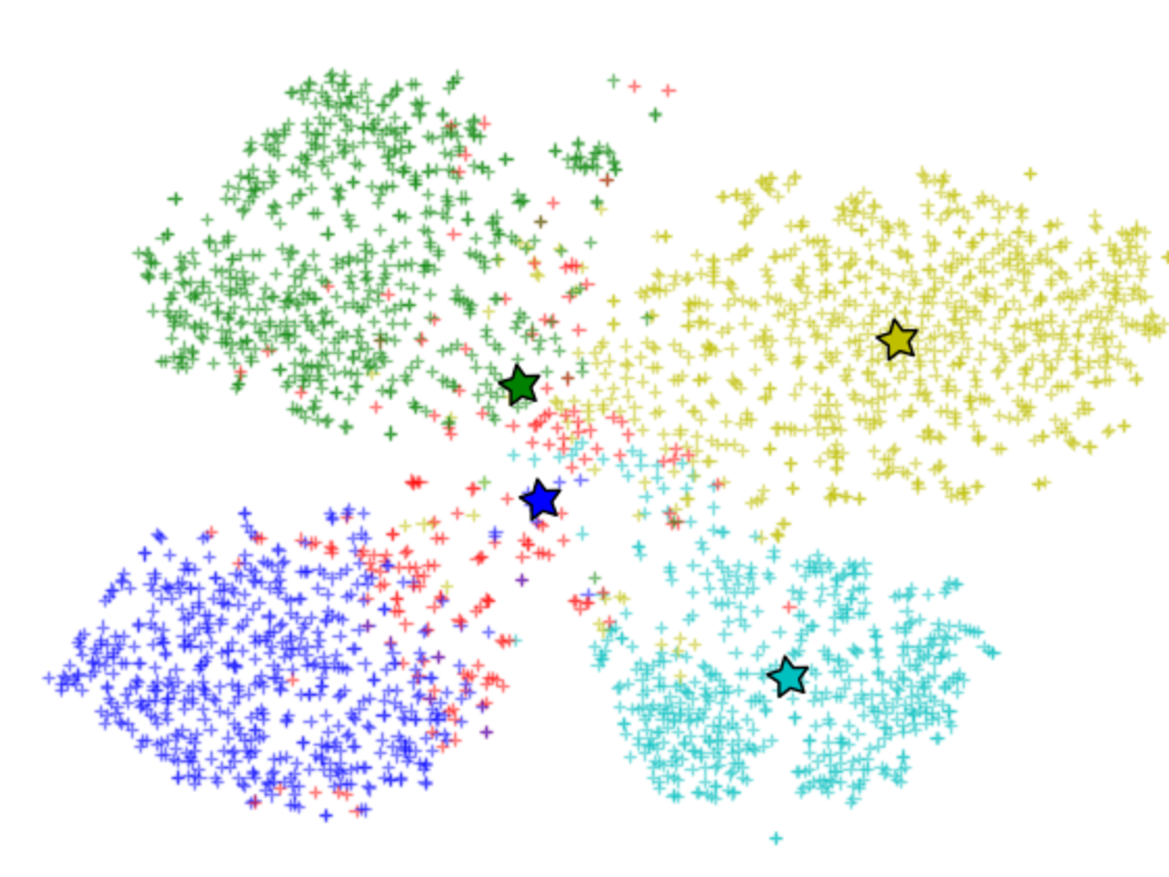
\includegraphics[width=\linewidth]{images/own_cluster}
    \caption{}
    \label{fig:clustering}
% \caption{Stars as previous. Classification by our compatibility function using our supervised clustering}
  \end{subfigure}
%
  \begin{subfigure}[b]{0.27\linewidth}
    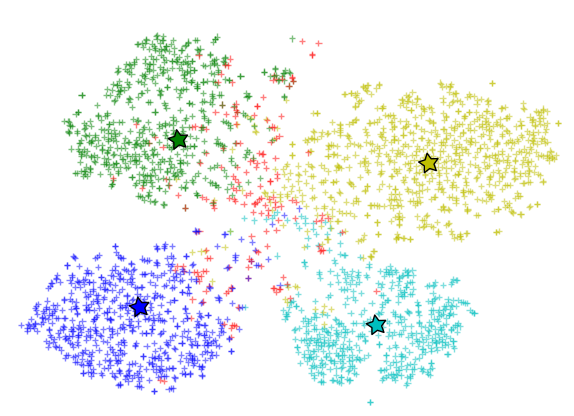
\includegraphics[width=\linewidth]{images/jeac}
    \caption{}
    \label{fig:jeac}
% \caption{Class signatures mapped to image space (stars) and cluster assignment by JEaC}
  \end{subfigure}
  \caption[تحلیل قسمت‌های مختلف روش پیشنهادی]{
  نمایش دوبعدی چهار دسته از مجموعه دادگان AwA با استفاده از نگاشت \lr{t-SNE}، دو دسته‌ی دیده شده شامل بزگوزن (فیروزه‌ای) خرس گریزلی (زرد) و دو دسته‌ی دیده نشده شامپانزه (آبی) و پاندا (سبز). تصاویر با نماد بعلاوه و نگاشت توصیف دسته‌ها در فضای تصاویر با ستاره نشان داده شده است. در تصاویر b تا f نقطه‌های قرمز نمونه‌هایی که را نشان می‌دهد که دسته‌ای به جز چهار دسته‌ی موجود در شکل برای آن‌ها پیش‌بینی شده است.
  \textbf{آ)}
   دسته‌های دیده شده با برچسب صحیح و دیده‌نشده با رنگ مشکی
\textbf{ب)}
 نمایش برچسب صحیح برای تمامی دسته‌ها
  \textbf{ج)} توصیف‌ها با نگاشت \eqref{eq:d_answer}
  به فضای تصاویر برده شده‌اند و دسته‌بندی با دسته‌بند نزدیک‌ترین همسایه انجام شده است.
  \textbf{د)}
   نگاشت مانند حالت قبل و دسته‌بندی با تابع مطابقت پیشنهادی به همراه خوشه‌بند \lr{k-means}
  \textbf{هـ)}
   نگاشت مانند حالت قبل و دسته‌بندی با تابع مطابقت پیشنهادی به همراه خوشه‌بند نیمه‌نظارتی پیشنهاد شده
  \textbf{و)}
  دسته‌بندی و نگاشت با استفاده از روش پیشنهادی برای یادگیری نگاشت و خوشه‌بندی توام
  }
\label{fig:discussion}
\end{figure}
